\documentclass[conference]{IEEEtran}
\IEEEoverridecommandlockouts
% The preceding line is only needed to identify funding in the first footnote. If that is unneeded, please comment it out.
\usepackage{cite}
\usepackage{listings} 
\usepackage{xcolor}
\lstset{
  language=Python,  
  frame=shadowbox, 
  rulesepcolor=\color{red!20!green!20!blue!20},
  keywordstyle=\color{blue!90}\bfseries, 
  commentstyle=\color{red!10!green!70}\textit,    
  showstringspaces=false,
  numbers=left, 
  numberstyle=\tiny,    
  stringstyle=\ttfamily, 
  breaklines=true, 
  extendedchars=false,  
  texcl=true}
\usepackage{amsmath,amssymb,amsfonts}
\usepackage{algorithmic}
\usepackage{graphicx}
\usepackage{float} 
\usepackage{subfigure} 
\usepackage{textcomp}
\usepackage{xcolor}
\def\BibTeX{{\rm B\kern-.05em{\sc i\kern-.025em b}\kern-.08em
    T\kern-.1667em\lower.7ex\hbox{E}\kern-.125emX}}
\begin{document}

\title{Project A:Visual Interpretation of Convolutional Neural Networks}
%{\footnotesize \textsuperscript{*}Note: Sub-titles are not captured in Xplore and should not be used}
%\thanks{Identify applicable funding agency here. If none, delete this.}


\author{\IEEEauthorblockN{Wenrui Xu}
\IEEEauthorblockA{\textit{1008313228}}
\and
\IEEEauthorblockN{Jiaming Xu}
\IEEEauthorblockA{\textit{1007698831}}
}

\maketitle

\begin{abstract}
\end{abstract}

\section{Task 1: 1-Dimensional digit classification}
\subsection{Question 1}
\begin{lstlisting}
    weight_decay = 5e-4
    model = Sequential()
    #Your code starts from here 
    model.add(Input(shape=(40,1)))
    model.add(Conv1D(25, kernel_size=5, padding='same', activation='relu', kernel_regularizer=regularizers.l2(weight_decay)))
    model.add(Conv1D(25, kernel_size=3, padding='same', activation='relu', kernel_regularizer=regularizers.l2(weight_decay)))
    model.add(Conv1D(25, kernel_size=3, padding='same', activation='relu', kernel_regularizer=regularizers.l2(weight_decay)))

    model.add(Flatten())
    model.add(Dense(10, activation='softmax', kernel_initializer=keras.initializers.RandomNormal(mean=0.0, stddev=0.5),
                    bias_initializer=keras.initializers.Zeros(), kernel_regularizer=regularizers.l2(weight_decay)))

    model.summary()
\end{lstlisting}
In this question, we build a ConvNet. It includes three convolutional layer, one flatten layer and one dense layer.
The network is listed as followed\ref{Fig.t1q1}:
\begin{figure}[H] 
    \centering %图片居中
    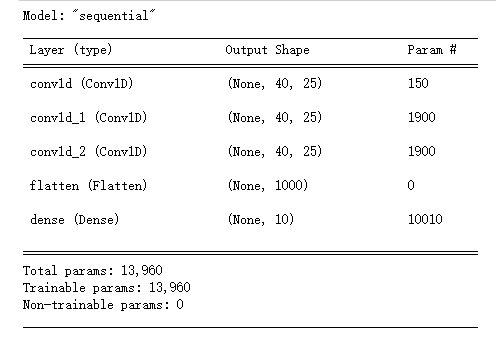
\includegraphics[width=0.7\textwidth]{T1Q1.png} %插入图片,[]中设置图片大小,{}中是图片文件名
    \caption{Task1-Question1: ConvNet Model} %最终文档中希望显示的图片标题
    \label{Fig.t1q1} %用于文内引用的标签
\end{figure}
\subsection{Question 2}
In this section, we apply the model in question 1 to the MNIST1D dataset. The code is listed as followed:
\begin{lstlisting}
    model.compile(loss=keras.losses.categorical_crossentropy,
              optimizer=tensorflow.keras.optimizers.SGD(),
              metrics=['accuracy'])

    def lr_scheduler(epoch):
        base_ep = 15
        return 1e-3 * (.5 ** (epoch // base_ep))
    lr_reduce_cb = keras.callbacks.LearningRateScheduler(lr_scheduler)
    tensorboard_cb = keras.callbacks.TensorBoard(log_dir='log2', write_graph=True)
    early_stopping_cb = keras.callbacks.EarlyStopping(patience=8, min_delta=0.)

    # X = tensorflow.expand_dims(dataset['x'],axis=2)
    train_x=dataset['x']
    train_y=dataset['y']
    train_x=train_x.reshape(4000,40,1)
    train_y=tensorflow.keras.utils.to_categorical(train_y, num_classes=10)

    # print(X.shape)
    history=model.fit(x=train_x,y=train_y,epochs=200,
    #                     steps_per_epoch=len(X) // 32,
                        callbacks=[tensorboard_cb],                  
                        shuffle = True,
                        verbose=1)
    model.save('MNIST1D.h5')
\end{lstlisting}
Here, we use the tensorboard to record the training procedure.First of all, we compile this model, set the loss function to cross-entropy, set the optimizer to Stochastic Gradient Descent and the metrics to accuracy. 
Then we define the LearningRateScheduler, the TensorBoard, the EarlyStopping for later use.
After that, we handle the train data for training.
At last, we will fit the data and tensorboard into the model for training and save the model into disk.
The training result is shown as followed\ref{Fig.t1q2}:
\begin{figure}[H] 
    \centering %图片居中
    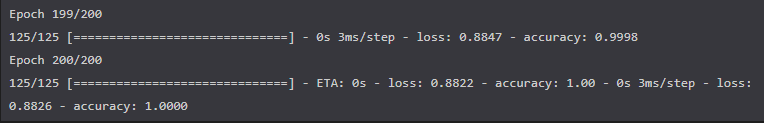
\includegraphics[width=0.7\textwidth]{T1Q2.png} %插入图片,[]中设置图片大小,{}中是图片文件名
    \caption{Task1-Question2: Training Results} %最终文档中希望显示的图片标题
    \label{Fig.t1q2} %用于文内引用的标签
\end{figure}
\subsection{Question 3}
\subsubsection{SubQuestion a}
\begin{lstlisting}
    train_acc = history.history['accuracy']
    train_loss = history.history['loss']
    plt.plot(train_acc)
    plt.figure()
    plt.plot(train_loss)
\end{lstlisting}
This is the code for loss and accuracy curve, the plot of loss curve\ref{Fig.t1q3a1} and plot for accuracy curve\ref{Fig.t1q3a2} are shown below:
\begin{figure}[H] 
    \centering %图片居中
    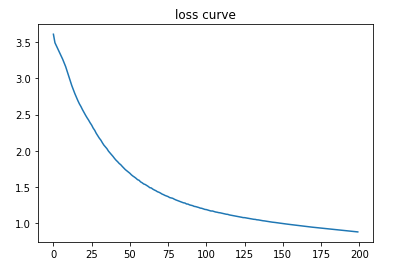
\includegraphics[width=0.7\textwidth]{T1Q3-b.png} %插入图片,[]中设置图片大小,{}中是图片文件名
    \caption{Task1-Question3a-1: loss curve} %最终文档中希望显示的图片标题
    \label{Fig.t1q3a1} %用于文内引用的标签
\end{figure}
\begin{figure}[H] 
    \centering %图片居中
    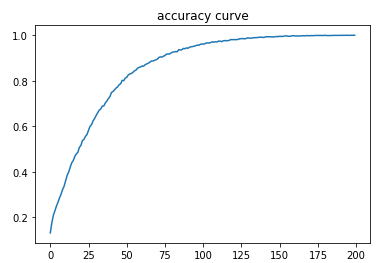
\includegraphics[width=0.7\textwidth]{T1Q3-a.png} %插入图片,[]中设置图片大小,{}中是图片文件名
    \caption{Task1-Question3a-2: accuracy curve} %最终文档中希望显示的图片标题
    \label{Fig.t1q3a2} %用于文内引用的标签
\end{figure}
\subsubsection{SubQuestion b}
This part talks about overall classification accuracy on the test set.

overall accuracy、 
\subsubsection{SubQuestion c}
class-wise accuracy
\subsubsection{SubQuestion d}
roc auc曲线
\subsubsection{SubQuestion e}
混淆矩阵
\subsubsection{SubQuestion f}
召回率,准确率和F-1得分

\subsection{Question 4}
挑几个正确与错误的例子,评价一下,哪两个类错误最多
\section{Task 2: CNN interprectation}
CNN方法实现
选择方法填补了什么空白,有什么贡献和创新点
所选方法算法细节
讨论主要优缺点,在不同场景下能否使用,方法能否分析之前的错误,为什么?

实现

\section{Task 3: Biomedical image classification and interpretation}
性能评价,并分析

方法用到HMT

CAPTUM可选项

\section{Task 4: Quantitative evaluation of the attribution methods}
应用,k设置为30,计算平均drop increase,HMT设置为90

讨论之前用过的方法,你的方法又没有正确反映特征,什么时候会失败,比较一下,给个reason


\begin{thebibliography}{00}
\bibitem{b1}Y. Gilad, R. Hemo, S. Micali, G. Vlachos, and N. Zeldovich, “Algorand: Scaling Byzantine Agreements for Cryptocurrencies,” in Proceedings of the 26th Symposium on operating systems principles, 2017, pp. 51–68. doi: 10.1145/3132747.3132757.
\bibitem{b2} King, Sunny, and Scott Nadal. "Ppcoin: Peer-to-peer crypto-currency with proof-of-stake." self-published paper, August 19.1, 2012.

\end{thebibliography}

\end{document}
